\chapter{POES/MetOp}
\label{app:poes}
POES/MetOp(Polar Orbiting Environmental Satellites/Meteorological Operational Satellites、以下POES衛星)はNOAA(アメリカ海洋大気庁: National Oceanic and Atmospheric Administration) Space Weather Prediction Centerによって開発・運用されており、太陽同期軌道で周回する衛星である~\cite{poes2013noaa}。
POES衛星にはSEM-2(Space Environment Monitor-2)という観測装置が搭載されており、TED(Total Energy Detector)とMEPED(Medium Energy Proton and Electron Detector)で構成される。
MEPEDは、高エネルギーイオンと高エネルギー電子のフラックスを測定しており、in situ観測で行われる。\par

高エネルギー電子の観測においては、4つのエネルギーバンドをもち($>40\ \mathrm{keV}$, $>130\ \mathrm{keV}$, $>287\ \mathrm{keV}$, $>612\ \mathrm{keV}$)、2つの角度(0\textdegree, 90\textdegree)のフラックスを測定する。
0\textdegree では天頂方向を向いて観測を行っており、90\textdegree では、0\textdegree に対して垂直であり、衛星の速度方向とは逆向きに設置されている~\cite{meped2013noaa}。\par

POES衛星は複数の衛星で構成されており、運用されいる衛星は時期によって異なる。
トロムソの\ce{NO}の柱密度の比較においては6基の衛星(METOP-01, METOP-02, METOP-03, NOAA-15, NOAA-18, NOAA-19)を用い、昭和基地の\ce{NO}の柱密度の比較においては5基の衛星(METOP-01, METOP-03, NOAA-15, NOAA-18, NOAA-19)を用いた。
POES衛星の観測データについては、\url{https://www.ngdc.noaa.gov/stp/satellite/poes/dataaccess.html}より取得した。\par

電子フラックスデータの選定においては、観測場所(トロムソ・昭和基地)付近に降り込んでくると予想されるものであるかどうかを観点において、以下の条件で行った。
\begin{enumerate}
    \item 0\textdegree の電子フラックスデータ
    \item L値
    \par
    L値(L-shellまたはL-value)とは、磁力線が磁気赤道を横切る際に、地球の中心からどの程度離れているかを地球の半径の何倍かで表したものである。
    本研究では、L値が$5.5-7.5$の範囲である電子フラックスデータを用いた

    \item MLT(Magnetic Local Time)とUT(Universal Time)
    \par
    MLTとは、一般に用いられる自転軸から定義されるLT(Local Time)とは異なり、地磁気極から定義されるものである。
    トロムソにおいてはMLTがUTに対して2.24時間進んでいて、昭和基地においてはUTと等しいと仮定した。
    これを踏まえて、条件にあうUTとMLTで観測された電子フラックスデータを用いた(図\ref{fig:app_poes_box})。
    図中の破線はMLTのUTに対する差の仮定に基づいて、$\mathrm{MLT}-\mathrm{UT}$軸のグラフに表したものである。
    この破線に沿って$\mathrm{MLT}\ 3h \times \mathrm{UT}\ 3h$のBoxを考える。
    このBox内に含まれる電子フラックスデータを用いる。
    \begin{figure}[htbp]
        \centering
        \begin{minipage}{.495\linewidth}
            \leftline{(a)}
            \centering
            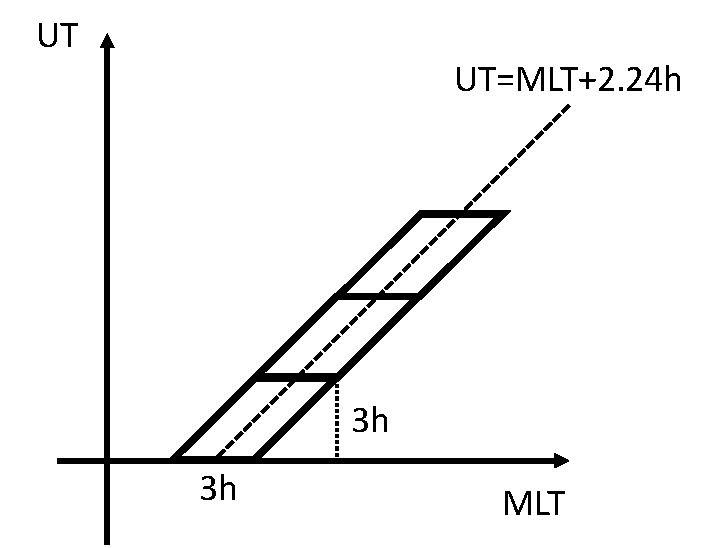
\includegraphics[scale=0.5]{master_thesis_contents/master_thesis_fig/app_poes_box_tromsoe.pdf}
        \end{minipage}
        \begin{minipage}{.495\linewidth}
            \leftline{(b)}
            \centering
            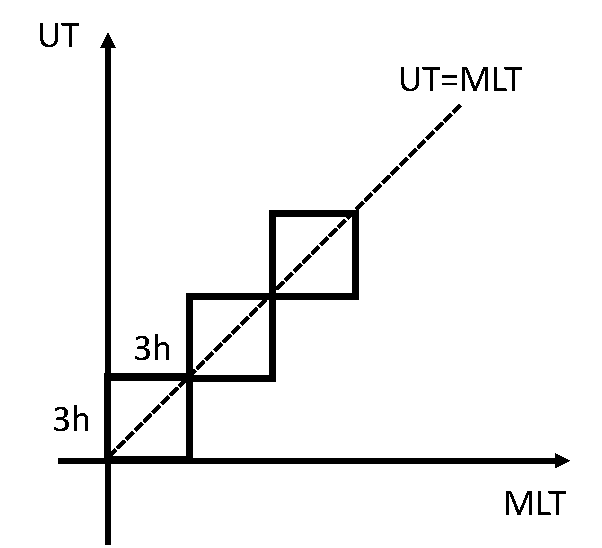
\includegraphics[scale=0.5]{master_thesis_contents/master_thesis_fig/app_poes_box_syowa.pdf}
        \end{minipage}
        \caption{電子フラックスデータの3時間平均の値の計算に用いるBox。(a) トロムソの場合。(b) 昭和基地の場合。}
        \label{fig:app_poes_box}
    \end{figure}
\end{enumerate} \par
以上の条件を満たした電子フラックスデータについて、図\ref{fig:app_poes_box}で示したBoxごとに平均値を計算し3時間平均値としてプロットを行った。
